\section{Lezione 6}%
\label{sub:Lezione 6}

\subsection{Modelli semplici di Random Walk}%
\label{sub:Random Walk}

Mettiamoci in una situazione unidimensionale, con un oggetto che può fare salti di ampiezza unitaria.
\usetikzlibrary{arrows.meta,bending}
\begin{center}
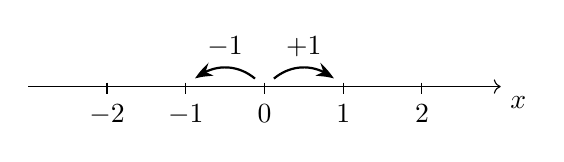
\begin{tikzpicture}[bullet/.style={circle,inner sep=0.7ex},x=2cm,auto,bend angle=40]
    \tikzmath{\x = 1.5; \z = 0;}
    \draw[->] (-\x,0) -- (\x,0) node[below right]{$x$};
    \path (-\x/3,0) node[bullet] (-a) {}
     (0,0) node[bullet] (0) {}
     (\x/3,0) node[bullet] (a) {};
    \foreach \Y [count=\X starting from -2] in {-2,-1,0,1,2} 
     {\draw (\X/2,0.05) -- (\X/2,-0.1) node[below]{$\Y$};}
    \draw[-{Stealth[bend]},thick] (0) to[bend left] node{$+1$} (a);
    \draw[-{Stealth[bend]},thick] (0) to[bend right] node[above]{$-1$} (-a);
\end{tikzpicture}
\end{center}

Possiamo analizzare due modelli di RW:
\begin{enumerate}
    \item Salto di $\pm 1$ ad un tempo casuale.
    \item Salto di $\pm 1$ ad un tempo $\tau$ fissato.
\end{enumerate}
Entrambi i casi descrivono processi Markoviani.
\subsubsection{1. Salto ad un tempo random.}%
\label{subsub:1. Salto ad un tempo random.}
L'equazione di Chapman-Kolmogorov in forma differenziale per il processo si scrive come:
\[\begin{aligned}
    \partial_{t}P\left(n,t|n',t'\right) = \left[ \ \right.&\omega\left(n|n+1,t\right)P\left(n+1, t|n',t'\right) +\\
                                             +& \omega\left(n|n-1,t\right)P\left(n-1, t|n',t'\right) + \\
					     -& \left. 2P\left(n,t|n',t'\right) \ \right]
.\end{aligned}\]
Facciamo chiarezza sui termini in equazione, prendiamo il primo nella parentesi quadra dopo l'uguale:
\[
    \omega\left(n|n+1,t\right)P\left(n+1, t|n',t'\right)
.\] 
Questo indica la probabilità di essere in $n+1$ (descritta dal termine $P$) e di fare un salto all'indietro (descritta dalla probabilità corrispondente $\omega$).\\
L'ultimo termine in parentesi indica la probabilità di essere in $n$ al tempo $t$, se ci troviamo in tal punto allora allo step successivo usciamo sicuramente fuori per costruzione del moto.\\
Imponendo che il rate di salto in avanti sia uguale a quello di salto all'indietro:
\begin{equation}
    \omega (n+1|n,t) = \omega (n-1|n,t) \equiv d \label{6_rate}
\end{equation}
Possiamo semplificare l'equazione del processo:
\begin{bluebox}{Chapman-Kolmogorov per RW 1.}
    \begin{equation}
\begin{aligned}
    \partial_{t}P\left(n,t|n',t'\right) = d\left[ \ \right.&P\left(n+1, t|n',t'\right) +\\
                                             +& P\left(n-1, t|n',t'\right) + \\
					     -& \left. 2P\left(n,t|n',t'\right) \ \right]
					     \label{eq:RW_1}
.\end{aligned}
    \end{equation}
\end{bluebox}
\noindent
Si risolve in trasformata:
\[
    G(s,t) = \left<e^{isn}\right> = \sum_{n}^{\infty} P\left(n,t|n',t'\right)e^{isn}
.\] 
Quando abbiamo un termine del tipo $P\left(n\pm 1|n',t'\right)$ basta scrivere:
\[
    e^{isn}P\left(n\pm 1, t|n',t'\right) = e^{\mp is} e^{is(n\pm 1)}P\left(n\pm 1, t|n',t'\right)
.\] 
Quindi inserendo nella equazione di CK:
\[
    \partial_{t}G(s,t) =d\left(e^{-is}+ e^{is}-2\right)G(s,t) 
.\] 
Si risolve per $G(s,t)$:
\[
    G(s,t) = \exp \left[\left(e^{is}+e^{-is}-2\right)td\right]G(s,0) 
.\] 
Andando a cercare la soluzione stazionaria si ha che:
\[
t\to \infty \implies s\to 0
.\] 
Questo per le relazioni tra spazio reale e trasformata: in sostanza stiamo assumendo i camminatori come oggetti reali, quindi se $\omega\to 0$ dev'essere necessariamente che $s\to 0$:
\[
    \omega  \sim sc
.\] 
Tornando alla $G$ sviluppando si ottiene una Gaussiana:
\[
    G(s,t) = \exp(-s^2td) 
.\] 

\subsubsection{2. Salto ad un tempo $\tau$ fissato}%
\label{subsub:2. Salto ad un tempo tau fissato}
In questo caso il tempo è una variabile discreta di passo $\tau$.
\begin{bluebox}{Equazione per il propagatore nel RW 2}
\begin{equation}
\begin{aligned}
    P\left(n,(N+1) \tau|\right.&\left.n',N'\tau\right)= \\
			       &\frac{1}{2}\left[P\left(n+1,N\tau|n',N'\tau\right)\right. + \\
			       & \quad + \left.  P\left(n-1,N\tau|n',N'\tau\right)\right] \label{eq:6_1}
.\end{aligned}
\end{equation}
    
\end{bluebox}
\noindent

\begin{greenbox}{RW1 e RW2 equivalenti per scale piccole.}
 Se $\tau$ è piccolo rispetto a $N\tau$ il caso (2) diventa equivalente al caso (1).   
\end{greenbox}
\noindent
Definiamo il tempo $t' = N'\tau$:
\begin{equation}
\begin{aligned}
    P\left(n,(N+1) \tau|n',N'\tau\right)\simeq & P\left(n,N\tau|n',t'\right) + \\
					       & + \tau\partial_{t}P\left(n,N\tau|n',t'\right) \label{eq:6_2}
.\end{aligned}
\end{equation}
Si procede definendo: 
\[
 d \equiv 1 /2\tau   
.\] 
Possiamo ottenere l'equazione \ref{eq:RW_1} sostituendo al primo termine della \ref{eq:6_1} il secondo della \ref{eq:6_2} .\\
Risolviamo adesso la \ref{eq:6_1} con il metodo della funzione caratteristica ($G(s,t) = \left<e^{ins}\right>$ ):
\[
    G(s, (N+1)\tau) = \frac{1}{2}\left(e^{is}+ e^{-is}\right)G(s,N\tau) 
.\] 
Come condizione iniziale si impone che $G(s,0) = 1$.\\
In questo modo l'equazione in $G$ è una ricorsiva in $N$ che ha soluzione:
\[
    G(s,N\tau) = \left(\frac{1}{2}\left(e^{is}+e^{-is}\right)\right)^{N}
.\] 
A questo punto possiamo vedere che se $N\to \infty$ si ottiene una soluzione Gaussiana come nell'RW1 (mandare $N\to \infty$ significa limite stazionario).
\[
    \begin{cases}
        \tau N = t\\
	d = \dfrac{1}{2\tau}
    \end{cases}
    \implies  
    \frac{td}{N} = \frac{1}{2}
.\] 
\[
    G(s,N\tau) = \left[1 + \frac{td}{N}\left(e^{is}+ e^{-is}-2\right)\right]^N
.\] 
Sfruttando il limite notevole:
\[
    \lim_{x \to \infty} \left(1+\frac{\alpha}{x}\right)^{x} = e^{\alpha}
.\] 
Si ottiene:
\[
    G(s, N\tau) \xrightarrow[]{N \to \infty} G(s,t) = \exp\left[td\left(e^{is}+e^{-is}-2\right)\right]
.\] 
In conclusione è come se, aspettando abbastanza a lungo, la caoticità sul salto di $\pm 1$ contagiasse il clock di salto $\tau$ rendendo anch'esso caotico come nel caso RW1.\\
Nel proseguo distingueremo i due casi solo dove necessario vista la loro equivalenza a stazionarietà.

\subsubsection{Limite al continuo nei salti}%
\label{subsub:Limite al continuo}
Definiamo lo spazio percorso dal camminatore dopo $n$ step in un reticolo di passo $l$:
\[
    x = nl
.\] 
\usetikzlibrary{arrows.meta,bending}
\begin{center}
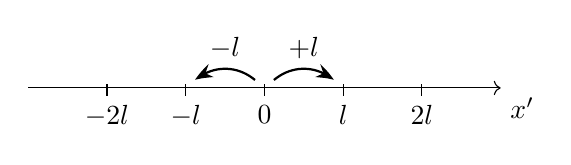
\begin{tikzpicture}[bullet/.style={circle,inner sep=0.7ex},x=2cm,auto,bend angle=40]
    \tikzmath{\x = 1.5; \z = 0;}
    \draw[->] (-\x,0) -- (\x,0) node[below right]{$x'$};
    \path (-\x/3,0) node[bullet] (-a) {}
     (0,0) node[bullet] (0) {}
     (\x/3,0) node[bullet] (a) {};
    \foreach \Y [count=\X starting from -2] in {-2l,-l,0,l,2l} 
     {\draw (\X/2,0.05) -- (\X/2,-0.1) node[below]{$\Y$};}
    \draw[-{Stealth[bend]},thick] (0) to[bend left] node{$+l$} (a);
    \draw[-{Stealth[bend]},thick] (0) to[bend right] node[above]{$-l$} (-a);
\end{tikzpicture}
\end{center}

Quello che faremo sarà far il limite per $l\to 0$.\\
La trasformata si modifica per questo caso nel seguente modo:
\begin{equation}
\begin{aligned}
    \phi (s,t) = &\left<e^{isx}\right> = G(ls, t) =\\
		 & = \exp \left[\left(e^{ils} + e^{-ils} -2 \right)td\right]
		 \label{eq:6_continuo}
.\end{aligned}
\end{equation}
Dove ricordiamo che $d$ è il rate del processo definito dalla \ref{6_rate}.\\
Si studia adesso anche il caso stazionario, quindi dobbiamo effettuare entrambi i limiti:
\[\begin{aligned}
    &l\to 0\\
    &\tau\to 0
.\end{aligned}\]
Sviluppando nell'esponenziale della \ref{eq:6_continuo} ci si rende conto che sopravvive solo il termine:
\[
    \sim \exp\left(-s^2l^2td\right)
.\] 
Per questo è necessario che:
\[
    D = \lim \limits_{\substack{%
	         l \to 0\\
		  d \to \infty}} l^2d = \text{Finito}
.\] 
Fare il limite per il Rate $d\to \infty$ è lo stesso che fare il limite per $\tau\to 0$ poiché per definizione $d = 1 /2\tau$.\\
In conclusione otteniamo un andamento per $\phi$ Gaussiano:
\begin{bluebox}{Funzione caratteristica per RW nel limite continuo}
\[
    \phi (s,t) = \exp\left(-s^2tD\right)
.\]     
\end{bluebox}
\noindent
Quindi abbiamo anche che:
\begin{equation}
    \left<x^2\right> \sim  2tD \label{eq:6_mom_sec}
\end{equation}
\subsubsection{Random Walk e processi di Wiener}%
\label{subsub:Random Walk e processi di Wiener}
Si può dimostrare che per $l\to 0$ l'equazione che regola il propagatore $P$ è una Fokker-Plank (che regola anche i processi di Wiener). \\
Partiamo dalla Master Equation già scritta sopra:
\[\begin{aligned}
    \partial_{t}P(n) = d\left(P(n+1) + P(n-1) -2 P(n) \right)
.\end{aligned}\]
Sviluppando in $l=0$ si ha:
\[\begin{aligned}
    &P(n+1) = P(n) + \partial_{x}P(n) l + \frac{1}{2}\partial^2_{x^2} l^2P(n) \\
    &P(n+1) = P(n) - \partial_{x}P(n) l + \frac{1}{2}\partial^2_{x^2} l^2P(n)
.\end{aligned}\]
E reinserendo nella equazione per $P$ si ha:
\[
    \partial_{t}P(n) = dl^2 \partial^2_{x^2} P(n) 
.\] 
Che è appunto una Fokker-Plank.

\subsection{Random Walk di Weierstrass}%
\label{sub:Random Walk di Weierstrass}
Questo RW è più complesso dei primi due, si basa su alcuni parametri che ne determinano il passo ed il rate: ($N$, $b$).\\
Adesso anziché fare salti fissi di $l$ si fanno salti $J_n$ con rate $R_n$ che variano al variare dell'intero $n$. $J_n$ e $R_n$ sono così definiti:
\[
    J_n = \left(N^{n}+1\right)l \qquad R_n = \frac{\gamma}{b^n} \qquad b,N > 1
.\] 
\[
    n \in \left[0\ldots\infty\right]
.\] 
\usetikzlibrary{arrows.meta,bending}
\begin{center}
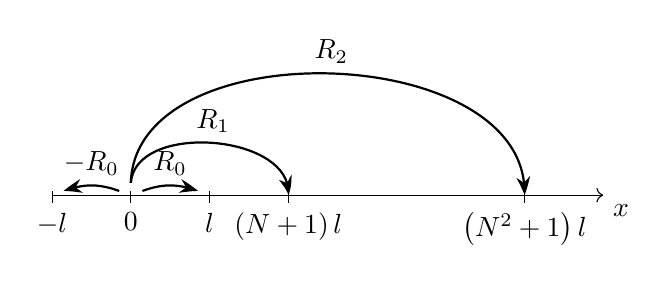
\begin{tikzpicture}[bullet/.style={circle,inner sep=0.7ex},x=2cm,auto,bend angle=40]
    \tikzmath{\x = 1.5; \z =3.; \w = 0.5;}
    \draw[->] (-\w,0) -- (\z,0) node[below right]{$x$};
    \path 
	(-\w,0) node[bullet] (-a) {}
        (0,0) node[bullet] (0) {}
        (\w,0) node[bullet] (a) {};
    \foreach \X\Y in {-\w/-l, 0/0, \w/l, 2*\w/\left(N+1\right)l , 5*\w/\left(N^2+1\right)l}
    { \draw (\X,0.05) -- (\X,-0.1) node[below]{$\Y$};}
    \draw[-{Stealth[bend]},thick] (0) to[bend right=20]node[above]{$-R_0$ } (-a);
    \draw[-{Stealth[bend]},thick] (0) to[bend left=20] node[above]{$R_0$ } (a);
    \draw[-{Stealth[bend]},thick] (0) to[bend left=90] node[above]{$R_1$} (2*\w,0);
    \draw[-{Stealth[bend]},thick] (0) to[bend left=90] node[above]{$R_2$ } (5*\w,0);
\end{tikzpicture}
\end{center}

Possiamo considerare $\gamma$ come il parametro corrispondente a $d$ della sezione precedente.
Quindi ad esempio si può avere:
\begin{itemize}
    \item Salto di $l$ con rate $\gamma$. 
    \item Salto di $\left(N+1\right)l$ con rate $\gamma  / b$.
    \item Salto di $\left(N^2+1\right)l$ con rate $\gamma /b^2$.
\end{itemize}
Come conseguenza salti più lunghi avranno rate più bassi (quindi saranno meno frequenti).\\
\subsubsection{Master Equation per il RW di Weierstrass}%
\label{subsub:Master Equation per il RW di Weierstrass}
\[\begin{aligned}
    \partial_{t}P\left(n,t|n',t'\right) = &\sum_{i=0}^{\infty} 
    \frac{\gamma}{b^{i}} \left[P\left(n+(N^{i}+1) ,t|n',t'\right) \right. + \\
		    & \qquad \quad + \left. P\left(n-(N^{i}+1) ,t|n',t'\right)\right] + \\
		     - &2 \sum_{i=0}^{\infty} \left(\frac{1}{b^{i}}\right) P\left(n,t|n',t'\right)
.\end{aligned}\]
La prima sommatoria tiene di conto di tutti i punti che possono arrivare da distanze diverse. La seconda sommatoria invece tiene conto di quelli che sono già nel punto e scappano via.\\
L'equazione descrive un processo a salti, di conseguenza il moto in questione è Markoviano. Come per gli altri RW risolviamo con la funzione caratteristica.
\[
    G(s,t) = \left<e^{isn}\right> = \sum_{n}^{\infty} e^{isn}P(n,t|n',t') 
.\] 
La master equation si riscrive come:
\[\begin{aligned}
    \partial_{t}G(s,t) = \gamma &\left[e^{is}\left( 1 + \sum_{n=0}^{\infty} \frac{e^{isN^{n}}}{b^{n}} \right) + \right.\\  
				& \ \ \left. + e^{-is}\left( 1 + \sum_{n=0}^{\infty} \frac{e^{-isN^{n}}}{b^{n}} \right) + \right.\\
				& \qquad \qquad \qquad \qquad \ \left.- 2 \sum_{n=0}^{\infty} \frac{1}{b^n} \right]G(s,t) 
.\end{aligned}\]
Possiamo compattare la scrittura con la notazione:
\[
    f(s) \equiv \left[e^{is}\left( 1 + \sum_{n=0}^{\infty} \frac{e^{isN^{n}}}{b^{n}} \right) + C.C - 2 \sum_{n=0}^{\infty} \frac{1}{b^n} \right]
.\] 
Che ci permette di esprimere direttamente il risultato:
\begin{bluebox}{Funzione caratteristica per il RW di Weierstrass}
\[
    G(s,t) = \exp\left(tf(s)\right)G(s,0) 
.\]     
\end{bluebox}
\noindent
\subsubsection{Limite stazionario}%
\label{subsub:Limite stazionario}
Vediamo se anche in questo caso mandando $t\to \infty$ si ottiene una Gaussiana come nei casi RW1 e RW2.\\
Sviluppando la $G$ per $s\to 0$ si ottiene che molti termini polinomiali si ammazzano a vicenda, rimane soltanto la seguente:
\[
    G(s,t) = \exp\left(-ts^2 \sum_{k=0}^{\infty} \left(\frac{N^2}{b}\right)^k\right)
.\] 
All'esponente notiamo che il coefficiente di diffusione $D$ è una sommatoria:
\[
    D \to \sum_{k=0}^{\infty} \left(\frac{N^2}{b}\right)^k\
.\] 
Quello che si scopre è quindi che il parametro $N^2 /b$ decide se il processo sarà Gaussiano o no, infatti:
\begin{redbox}{}
\begin{itemize}
    \item Se $N^2 /b< 1$ abbiamo una serie geometrica all'esponenziale che ci riconduce ad una forma Gaussiana.
    \item Se $N^2 /b > 1$ la sommatoria diverge, il processo resta Markoviano ma non vale più il teorema del limite centrale.
\end{itemize}
\end{redbox}
\noindent
Visto che il momento secondo è proporzionale a $D$ (eq. \ref{eq:6_mom_sec}) se ne conclude un processo con $N^2 /b > 1$ ha varianza infinita.\\
La cosa interessante è che abbiamo scoperto un processo random che al limite non diventa una Gaussiana \footnote{il momento secondo deve essere definito nelle ipotesi per il teorema del limite centrale\ldots}

\subsection{Random Telegraph}%
\label{sub:Random Telegraph}
Il RT è un processo random che coinvolge un sistema a due stati (o livelli):
\usetikzlibrary{math}
\tikzmath{\x = 5; \y = 0.5; \Y = 2;}
\begin{center}
\begin{tikzpicture}
     \draw[-stealth] (0,0) node[below]{$0$}-- (\x,0) node[right]{$t$};
     \draw[-stealth] (0,0) -- (0,\y)node[left]{$b$} -- (0,3*\y)node[left]{$a$} -- (0,\Y) node[above]{$RT$};
     \draw[thick] (0,\y) -- 
		  (1,\y);
     \draw[dotted](1,\y) --  
                  (1, 3*\y);

     \draw[thick] (1,3*\y) -- 
		  (2,3*\y);
     \draw[dotted](2,3*\y) --  
                  (2, \y);

     \draw[thick] (2,\y) -- 
		  (2.5,\y);
     \draw[dotted](2.5,\y) --  
                  (2.5,3*\y);

     \draw[thick] (2.5,3*\y) -- 
		  (4,3*\y);
     \draw[dotted](4,3*\y) --  
                  (4,\y);

     \draw[thick] (4,\y) -- 
		  (5,\y);

\end{tikzpicture}
\end{center}
\noindent

Il processo è descritto dalle equazioni differenziali:
\[\begin{aligned}
    &\partial_{t}P\left(a,t|x,t_0\right) = -\lambda P\left(a,t|x,t_0\right) + \mu P\left(b,t|x,t_0\right)\\
    &\partial_{t}P\left(b,t|x,t_0\right) = \lambda P\left(a,t|x,t_0\right) - \mu P\left(b,t|x,t_0\right)
.\end{aligned}\]
In cui $x$ può essere $a$ oppure $b$.\\
In questo caso c'è anche una terza equazione per la normalizzazione del processo:
\[
    P\left(a,t|x,t_0\right)+ P\left(b,t|x,t_0\right) = 1
.\] 
Si scelgono le condizioni iniziali:
\[
    P\left(x,t_0|x',t_0\right) = \delta_{xx'}
.\] 
E quello che si ottiene risolvendo le equazioni differenziali è:
\begin{equation}
    P\left(x', t|x,t_0\right) =  \frac{\omega (x') }{R} + e^{-R (t-t_0)}\left(\frac{\lambda}{R}\delta_{ax} + \frac{\mu}{R}\delta_{bx}\right)
    \label{eq:6_RT}
\end{equation}
In cui $R$ è la somma dei due rate:
\[
    R = \mu +\lambda
.\] 
Mentre la funzione $\omega (x')$ differenzia i casi con $x'=a$ e $x'=b$:
\[
    \omega(x') =
    \begin{cases}
        \lambda  \quad \text{ se } x' = a\\
        \mu  \quad \text{ se } x' = b
    \end{cases}
.\]
Il primo termine nella \ref{eq:6_RT} è il termine stazionario. Il secondo termine invece decade esponenzialmente in $t$, il termine con le  $\delta$  a moltiplicare deriva dalle condizioni iniziali inserite.
\[\begin{aligned}
    \left<x(t) | \left[x_0,t_0\right]\right> = & \sum_{x = a,b}^{} xP\left(x,t|x_0,t_0\right) = \\
					      = &\mathcal{R} + \left(x-\mathcal{R}\right)e^{-R(t-t_0)}
.\end{aligned}\]
Dove $\mathcal{R}$ è il Rate ridotto:
\[
\mathcal{R} = \frac{ a\mu + b\lambda}{\lambda + \mu}; \qquad R = \mu + \lambda
.\] 
Si può anche calcolare la varianza di $x(t)x(s)$, senza esplicitare i conti si ha:
\[\begin{aligned}
    \text{var}(x(t) x(s) ) = & \left<x(s) x(t) \right> - \left<x(s)\right>\left<x(t) \right> = \\
			     =& \frac{\left(a-b\right)^2\lambda\mu}{\mu +\lambda}e^{-R(t-t_0) }
.\end{aligned}\]
\begin{bluebox}{RT e OU}
    Le dipendenze dal tempo di media e varianza calcolate per il processo di Ornstein-Uhlenback sono le stesse che per il processo di Random Telegraph.
\end{bluebox}
\noindent
Per questo motivo spesso si preferisce studiare alcuni processi con il random telegraph che, analiticamente, permette di trovare la soluzione in modo più semplice.

\subsection{Integrali stocastici}%
\label{sub:Integrali stocastici}
Sia $x$ una variabile stocastica, il differenziale di questa variabile lo definiamo come:
\begin{equation}
    dx = d\omega (t) \label{eq:6_int}
\end{equation}
Ipotizziamo che il processo stocastico sia un processo di Wiener, in tal caso:
\[
    P(d\omega) \sim \exp\left(-\frac{\left(d\omega\right)^2}{dt}\right)
.\] 
Con $dt$ differenziale temporale.\\
Prendiamo allora una funzione $G(s)$, vogliamo definire cosa significa calcolare l'integrale di $G(s)$ se la misura è stocastica.
\begin{figure}[H]
    \centering
    \incfig{lez_6_int}
    \caption{\scriptsize Funzione $G(t)$ con punti stocastici $\omega_i$, $\Delta\omega_i$ è la distanza sull'asse $y$ tra il punto $\omega_{i-1}$ e $\omega_i$.}
    \label{fig:lez_6_int}
\end{figure}
Definiamo allora l'integrale come:
\begin{redbox}{Integrale stocastico}
\[
    \int_{t_0}^{t_n} G(s) d\omega (s) \equiv \lim^{\text{ms}}_{n \to \infty} \sum_{i}^{} G(\tau_i) \left[\omega (t_i) - \omega (t_{i-1}) \right]
\]     
Il valore dell'integrale dipende dalla scelta dei $\tau_i$.
\end{redbox}
\noindent
\'E interessante utilizzare come $G(t)$ il processo di Wiener stesso per vedere cosa succede:
\[
    G(t) = \omega (t) 
.\]
Inoltre definiamo gli step $\tau_i$ come:
\[\begin{aligned}
    \tau_i = t_{i-1} + \alpha (t_i - t_{i-1}) \qquad 0 <\alpha <1 \label{eq:tau}
.\end{aligned}\]
Valutiamo la sommatoria all'interno della definizione:
\[\begin{aligned}
    \left<S_n\right> =& \sum_{i=0}^{n} \left<\omega (\tau_i)\left[ \omega (t_i) - \omega (t_{i-1})  \right] \right>=\\
		      & = \sum_{i=0}^{n} \left<\omega (t_{i-1} +\alpha (t_i-t_{i-1}) ) \omega(t_i) \right> + \\
		  & \qquad \qquad - \left<\omega (t_{i-1} +\alpha (t_i-t_{i-1}) ) \omega(t_{i-1}) \right>
.\end{aligned}\]
Ricordando che nei processi di Wiener vale:
\[
    \left<\omega (t) \omega (s) \right> = \text{min}(s,t) 
.\] 
Rimane soltanto:
\[\begin{aligned}
    \left<S_n\right> =& \sum_{i=0}^{n} t_{i-1} + \alpha (t_i-t_{i-1}) -\sum_{i=0}^{n} t_{i-1} = \\
		      & =\alpha(t_n-t_0) 
.\end{aligned}\]
Di conseguenza con la scelta \ref{eq:tau} per i $\tau_i$ contano solo l'istante finale ed iniziale. \\
Inoltre quando $\alpha =0$ l'integrale si annulla, mentre quando $\alpha =1$ l'integrale è l'intervallo temporale.\\
La vera domanda da porsi è quale sia il giusto valore di $\alpha$\ldots
\subsection{Integrale di $\hat{\text{I}}$to e di Stratonovich}%
\label{sub:Integrale di Ito e di Stratonovich}
\subsubsection{Integrale di $\hat{\text{I}}$to}%
\label{subsub:Integrale di Ito}
$\hat{\text{I}}$to è un matematico Giapponese, integrare con $\hat{\text{I}}$to implica scegliere $\tau_i$ all'inizio dell'intervallo.
\begin{bluebox}{Integrale di $\hat{\text{I}}$to}
    \[
        \alpha  = 0
    .\] 
    \[
	\tau_i = t_{i-1}
    .\] 
\end{bluebox}
\noindent
Le somme parziali con questo integrale si scrivono come:
\[
    S_n = \sum_{i}^{} \omega (t_{i-1}) \left[\omega (t_i) -\omega (t_{i-1}) \right]
.\]
L'integrazione di $\hat{\text{I}}$to forma una \texttt{Martingala}.
\paragraph{Martingala}%
\label{par:Martingala}
Dato un set di variabili stocastiche:
\[
    \left\{x_i\right\}: E(\left|x_i\right|) < \infty
.\] 
\[
    \left\{x_i\right\} \text{ è marting.} \iff
    E(x_{n+1}|x_1,\ldots,x_n) = x_n
.\] 
Con $E$: valore di aspettazione.\\
Possiamo notare che il processo di Wiener realizza una martingala perché rispetta questa proprietà.\\
Il calcolo di $\hat{\text{I}}$to è anche non anticipante:
\begin{redbox}{Funzione non anticipante}
    $G(t)$ è non anticipante se è indipendente dall'incremento $\omega (t) - \omega (s) $ $\forall t, s$.
\end{redbox}
\noindent
\begin{exmp}[Esempi di funzioni non anticipanti]
    Dato un processo di Wiener $\omega (t)$ tutte le seguenti funzioni sono non anticipanti:
    \begin{itemize}
	\item $\omega (t) $.
	\item $\int dt f(\omega (t) ) $.
	\item $\int d\omega f(\omega (t) ) $.
    \end{itemize}
\end{exmp}
\noindent
\subsubsection{Integrale di Stratonovich}%
\label{subsub:Integrale di Stratonovich}
Stratonovich era un fisico russo, integrare con Stratonovich implica scegliere il centro dell'intervallo.
\begin{bluebox}{Integrale di Stratonovich}
    \[
        \alpha = \frac{1}{2}
    .\] 
    \[
        \tau_i = \frac{1}{2}\left(\tau_{i-1}+ \tau_i\right)
    .\] 
\end{bluebox}
\noindent
Le somme parziali in questo caso si scrivono come:
\[
    S_n = \sum_{i}^{} \omega\left(\frac{t_i + t_{i-1}}{2}\right)\left[\omega (t_i) -\omega (t_{i-1}) \right]
.\] 
L'integrale di Stratonovich ha caratteristiche analoghe a quello che si usa normalmente in fisica, infatti si applica bene con funzioni "morbide".

\begin{exmp}[]
    \[
	\int_{0}^{t} \omega (t) dt = 
	\begin{cases}
	    \dfrac{\omega^2(t)}{2}-\dfrac{\omega^2(0)}{2} = \dfrac{t}{2} & \text{ Strato}\\
	    \sum_{}^{} \omega_{i-1}\left(\omega_i-\omega_{i-1}\right) = 0 & \text{ }\hat{\text{I}}\text{to}
	\end{cases}
    \] 
\end{exmp}
\noindent

\subsection{Relazione tra l'incremento stocastico e l'incremento temporale.}%
\label{sub:Relazione tra l'incremento stocastico e l'incremento temporale.}
La relazione tra i due differenziali è la seguente:
\begin{greenbox}{}
\[
    \left(d\omega\right)^2\sim dt
.\] 
\end{greenbox}
\noindent
Questo significa che $d\omega$  è continuo ma non è differenziabile. Abbiamo già accennato alla non differenziabilità dei processi di Wiener, ecco un'altra riprova.\\
Tutti gli ordini più alti dell'incremento si annullano:
\[
    d\omega^{N+2} \sim 0 \qquad \forall N>0
.\] 
Più formalmente, consideriamo il seguente integrale:
\[\begin{aligned}
    \int\left(d\omega\right)^{2+N}G(t) = \lim^{\text{ms}}_{n \to \infty} \sum_{i=0}^{n} G_{i-1} (\Delta\omega_i)^{2+N} 
.\end{aligned}\]
Quello che si può dimostrare è che:
\[
  \lim^{\text{ms}}_{n \to \infty} \sum_{i=0}^{n} G_{i-1} (\Delta\omega_i)^{2+N} = 
  \begin{cases}
      \int dtG(t) & N=0\\
      0          & N>0 
  \end{cases}
\] 
Quindi anche che:
\[
    \int\left(d\omega\right)^2 G(t) = \int dtG(t) 
.\] 
\begin{redbox}{}
    \begin{equation}
	d\omega  \sim O(dt^{1 /2}) \label{eq:6_order}
    \end{equation}
\end{redbox}
\noindent
\subsubsection{Applicazione: Differenziale di una funzione}%
\label{subsub:Applicazione: Differenziale di una funzione}
Prendiamo una funzione del tempo e del processo di Wiener: $f\left[\omega,t\right]$. Visto che si ha la \ref{eq:6_order} il differenziale $df$  all'ordine più basso è:
\begin{bluebox}{Differenziale di una funzione}
    \[
	df\left[\omega,t\right] = \left[\frac{\partial d}{\partial t} + \frac{1}{2}\frac{\partial ^2 f}{\partial \omega^2} \right]dt + \frac{\partial f}{\partial \omega} d\omega
    .\] 
\end{bluebox}
\noindent
Questa struttura per il differenziale di una funzione è profondamente legata alla formula di $\hat{\text{I}}$to.
\subsection{Formula di $\hat{\text{I}}$to}%
\label{sub:Formula di ITO}
Supponiamo di avere una SDE della seguente forma:
\[
    dx = a(x,t) dt + b(x,t) d\omega
.\] 
La soluzione formale è del seguente tipo:
\[
    x(t) = x_0 + \int_{t_0}^{t} a(x,s) ds + \int_{t_0}^{t} b(x,s) d\omega (s)   
.\] 
Supponiamo che esista una ed una sola soluzione non anticipante
\footnote{Le ipotesi per cui vale sono negli appunti}. \\
Allora se ho una $f(x,t)$ con $x$ soluzione della SDE scrivendone il differenziale all'ordine più basso si ha:
\begin{redbox}{Formula di $\hat{\text{I}}$to}
    \[\begin{aligned}
	df(x,t) = 
	\left[\frac{\partial f}{\partial t} + 
	a \frac{\partial f}{\partial x} +
        \frac{1}{2}b^2 \frac{\partial ^2 f}{\partial x^2} \right] dt +
	b\frac{\partial f}{\partial x} d\omega 
    .\end{aligned}\]
    con $dx = adt + bd\omega$.
\end{redbox}
\noindent
L'utilità della formula è che ci permette di fare cambi di variabili con funzioni dipendenti da una variabile casuale.
\clearpage
